\begin{frame}
	\frametitle{GPIO Keyboard}
	\centering
	\begin{tikzpicture}
		\node at (-4,2) {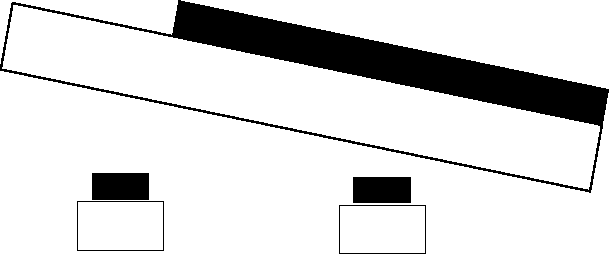
\includegraphics[width=4cm]{img/key1.pdf}};
		\node[align=left ,text width=4cm] at (1,2) { Two buttons connected \\ to GPIO ports};
		\node at (-4,0) {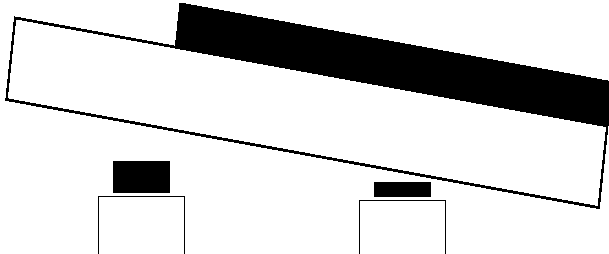
\includegraphics[width=4cm ]{img/key2.pdf}};
		\node[align=left ,text width=4cm] at (1,0) { Interrupt Time A};
		\node at (-4,-2) {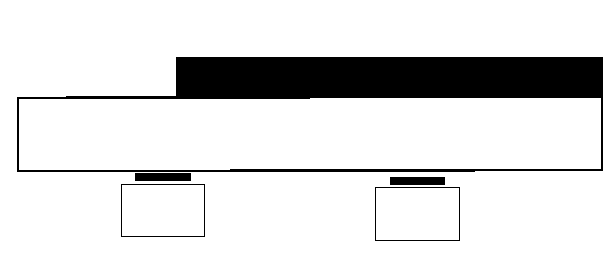
\includegraphics[width=4cm]{img/key3.pdf}};
		\node[align=left ,text width=4cm] at (1,-2) { Interrupt Time B};
		\node[align=left ,text width=6cm] at (-1,-3.5) {  $midi\_velocity=\frac{idle\_stroke}{Time B - Time A}$};
	\end{tikzpicture}	
	
\end{frame}
